\documentclass[12pt,table]{article}
\usepackage[table]{xcolor}
\usepackage{graphicx} % for including figure 
\usepackage{geometry} % geometry package for mentioning margin length
\usepackage{hyperref}
\usepackage{amssymb}
\usepackage{amsmath}
\usepackage{wrapfig}
\usepackage{listings}
\usepackage{xcolor}
\usepackage{sectsty}
\usepackage{color}

\usepackage{booktabs}

\renewcommand{\arraystretch}{1.2}




\lstdefinestyle{mystyle}{                 
    captionpos=b}
\lstset{style=mystyle}

\makeatletter
\newcommand\BeraMonottfamily{%
	\def\fvm@Scale{0.85}% scales the font down
	\fontfamily{fvm}\selectfont% selects the Bera Mono font
}

\makeatother
\definecolor{gray}{rgb}{0.4,0.4,0.4}
\definecolor{darkblue}{rgb}{0.0,0.0,0.6}
\definecolor{cyan}{rgb}{0.0,0.6,0.6}
\definecolor{maroon}{rgb}{0.5,0,0}
\definecolor{darkgreen}{rgb}{0,0.5,0}
\definecolor{ForestGreen}{RGB}{34,106,46}
\definecolor{lightgray}{rgb}{0.97, 0.97, 0.97}

\lstdefinelanguage{minizinc}{
	morekeywords={
		%% MiniZinc keywords
		%%
		ann, annotation, any, array, assert,
		bool,
		constraint,
		else, elseif, endif, enum, exists,
		float, forall, function,
		if, in, include, int,
		list,
		minimize, maximize,
		of, op, output,
		par, predicate,
		record,
		set, solve, string,
		test, then, tuple, type,
		var,
		where,
		%% MiniZinc functions
		%%
		abort, abs, acosh, array_intersect, array_union,
		array1d, array2d, array3d, array4d, array5d, array6d, asin, assert, atan,
		bool2int,
		card, ceil, combinator, concat, cos, cosh,
		dom, dom_array, dom_size, dominance,
		exp,
		fix, floor,
		index_set, index_set_1of2, index_set_2of2, index_set_1of3, index_set_2of3, index_set_3of3,
		int2float, is_fixed,
		join,
		lb, lb_array, length, let, ln, log, log2, log10,
		min, max,
		pow, product,
		round,
		set2array, show, show_int, show_float, sin, sinh, sqrt, sum,
		tan, tanh, trace,
		ub, and ub_array,
		%% Search keywords
		%%
		bool_search, int_search, seq_search, priority_search,
		%% MiniSearch keywords
		%%
		minisearch, search, while, repeat, next, commit, print, post, sol, scope, time_limit, break, fail
	},
	sensitive=true, % are the keywords case sensitive
	morecomment=[l][\em\color{ForestGreen}]{\%},
	%morecomment=[s]{/*}{*/},
	morestring=[b]",
}

\lstset{ %
	backgroundcolor=\color{lightgray},  % choose the background color; you must add
	% \usepackage{color} or \usepackage{xcolor}
	basicstyle=\scriptsize\ttfamily,    % the size of the fonts that are used for the code
	belowskip=-2em,
	breakatwhitespace=false,            % sets if automatic breaks should only happen at whitespace
	breaklines=true,                    % sets automatic line breaking
	captionpos=b,                       % sets the caption-position to bottom
	commentstyle=\color{ForestGreen},   % comment style
	%deletekeywords={...},              % if you want to delete keywords from the given language
	escapeinside={\%*}{*)},             % if you want to add LaTeX within your code
	extendedchars=true,                 % lets you use non-ASCII characters; for 8-bits
	% encodings only, does not work with UTF-8
	frame=single,                       % adds a frame around the code
	keepspaces=true,                    % keeps spaces in text, useful for keeping indentation
	% of code (possibly needs columns=flexible)
	keywordstyle=\bfseries\color{blue}, % keyword style
	language=minizinc,                  % the language of the code
	%morekeywords={*,...},              % if you want to add more keywords to the set
	numbers=left,                       % where to put the line-numbers; possible values are (none, left, right)
	%numbersep=5pt,                     % how far the line-numbers are from the code
	%numberstyle=\tiny\color{Gray},     % the style that is used for the line-numbers
	rulecolor=\color{black},            % if not set, the frame-color may be changed
	% on line-breaks within not-black text (e.g. comments (green here))
	showspaces=false,                   % show spaces everywhere adding particular
	% underscores; it overrides 'showstringspaces'
	showstringspaces=false,             % underline spaces within strings only
	showtabs=false,                     % show tabs within strings adding particular underscores
	%stepnumber=1,                      % the step between two line-numbers. If it's 1, each line will be numbered
	stringstyle=\color{Red},            % string literal style
	tabsize=1,                          % sets default tabsize to 2 spaces
	title=\lstname                      % show the filename of files included with \lstinputlisting;
	% also try caption instead of title
}

\hypersetup{
    colorlinks=true,
    linkcolor=blue,
    filecolor=magenta,	    
    urlcolor=cyan,
		citecolor=black,
}
\urlstyle{same}
\geometry{margin=3cm} %for setting margin; DON'T CHANGE THIS

\usepackage{bbm}
\usepackage{mathtools}
\usepackage{algorithm}
\usepackage{circuitikz}
%\usepackage{minted}
\usepackage[noend]{algpseudocode}
% the boxed option keeps the algorithm in a box in the pdf.
% You can also use the option ruled or algoruled for a different output.
% For more information about the algorithm2e package you can read the docuemntation 
% at https://mirror.easyname.at/ctan/macros/latex/contrib/algorithm2e/doc/algorithm2e.pdf

\newcommand{\BigO}{\ensuremath{\mathcal{O}}}
\title{Solving the Maze Problem with Inductive Logic Programming: A comparison between HYPER, Metagol and ILASP}
\author{Angelo Andreussi, Alex Della Schiava, Claudia Mau\ss ner}
\date{July 5, 2021}

\begin{document}
\maketitle

\section{Outline}
In this document, we intend to describe our Inductive Logic Programming (ILP) solutions to the Maze problem.\\
Section~\ref{sec:intro} offers a brief illustration of the Maze Problem we have been working on,
including the main choices and assumptions we made.\\
Section~\ref{sec:back} lists the tools we have used to reach our goal.

\section{Introduction}\label{sec:intro}

\begin{figure}[b]
    \centering
    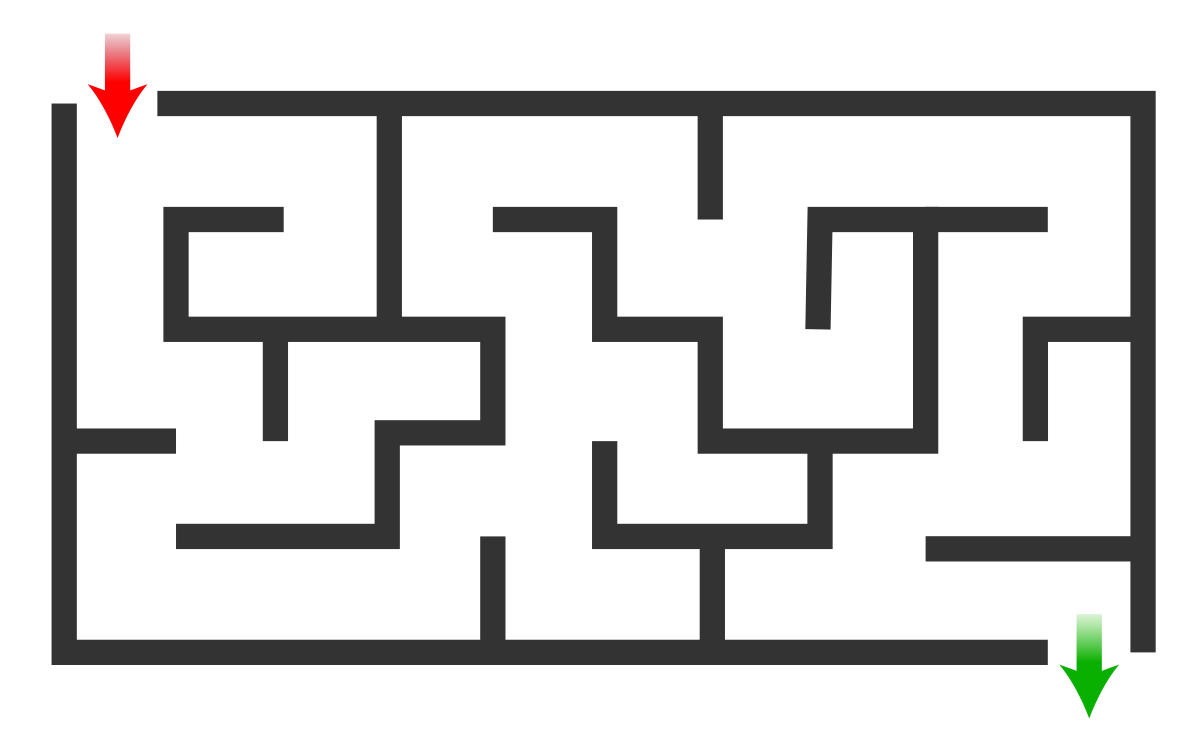
\includegraphics[scale=0.1]{img/Maze_simple.svg.png}
    \caption{Example of a Maze}\label{fig:fig1}
\end{figure}

The main objective of this project is to use different Inductive Logic Programming (ILP) techniques on the same problem in order to highlight
their differences. Despite the importance of performance differences (see Section~\ref{sec:perf}), we are also going to focus on the differences
concerning the approach to the problem, as some of us had to take completely different paths in order to reach similar goals.\\

Our work is focussed on the Maze problem. This problem consists in finding a path from point \texttt{A}
to point \texttt{B} in a labirinth-like shaped map (see Figure~\ref{fig:fig1}). A variety of classical algorithms
can be used to solve this problem, starting from the most naïve wall following algorithm to more complex and elaborated
ones exploiting graph theory concepts.\\
By approaching this simple problem with ILP though, it is possible to extend it into a much more sophisticated and interesting
problem. For instance, it allowed us to start with the assumption that the problem's main character (the
one we shall refer to as \emph{agent}) has no knowledge about \emph{how} to move. Consequently, before even trying
to solve the Maze, the agent needs to \emph{learn} what a \emph{move} is and, more specifically, what a \emph{legal} move is. The second
step consisted into \emph{teaching} the agent how to reach two distant cells. Lastly, in order to solve the Maze, it is either possible
to keep using ILP in order to find a solution or use the learned rules in order to implement them in a logic programming model of the planning
problem.\\
\section{Background}\label{sec:back}

\subsection{HYPER}
HYPER (Hypotheses refiner) is an ILP program, which has been developed by Prof. Dr. Ivan Bratko in 1999.\\
The following inputs must be given to the tool:
\begin{itemize}
    \item \textbf{Background Knowledge \((BK)\).} A set of logic formulas from which the positive examples can be derived.
    \item \textbf{Replacement of structured terms \((T)\).} Knowledge of how to refine structured terms like lists or coordinates.
    \item \textbf{Start clause \((S)\).} The starting hypothesis, which will be refined. 
    \item \textbf{Positive Examples \((E^+)\).}
    \item \textbf{Negative Examples \((E^-)\).}
\end{itemize}
The learning procedure is as follows:
\begin{itemize}
    \item \textbf{Choose a start hypothesis.} It is important to choose it general enough to be complete (i.e. cover all positive examples).
    \item \textbf{Continuously refine the hypothesis by:} 
	\begin{enumerate}
	\item Matching two variables of the same type or
	\item Adding a goal from the background knowledge or
	\item Refining a variable to background terms
	\end{enumerate}
\end{itemize}
Details on HYPER can be found in "Prolog Programming for Artificial Intelligence" by Ivan Bratko (4th edition, chapter 21).
\subsection{Metagol}
Metagol is a system used for ILP, which relies on meta-interpretative learning.\\
Using Metagol, four key components need to be defined:
\begin{itemize}
    \item \textbf{Metarules \((M)\).} Metarules are used to define the \emph{language bias} of the task. A large number metarules allows for a less strict language bias, hence a larger search space in which to find a solution. 
    \item \textbf{Background Knowledge \((BK)\).} The knowledge the system is initially assumed to have about the task to be carried out. It is a set of Prolog rules that the system can use either directly or indirectly in order to induce the hypothesis.
    \item \textbf{Positive Examples \((E^+)\).}
    \item \textbf{Negative Examples \((E^-)\).}
\end{itemize}
With these four components defined, Metagol will try to find a solution running the following algorithm:
\begin{enumerate}
    \item Select a positive example to be proven.
    \item Try to prove the example using the existing \(BK\) or previously induced clauses.
    \item (If step 2 did not work) Unify the example with the head of a metarule and repeat steps 1,2 and 3 for each atom in the body of the obtained rule.
    \item Once the hypothesis is proven to be complete (all the positive examples have been proven and covered), test its consistency. If any negative example is covered, backtrack to a choice made in step 3 which, supposedly, led to this situation.
\end{enumerate}
In this brief illustration of Metagol, the process of \emph{predicate invention} is not covered due to a lack of time to further study it. Our findings about this process mainly derive
from experimental experience and have no theoretical backup. Nonetheless, we will still point out the influence it had on our results.


\subsection{ILASP}

ILASP enables learning programs containing normal rules, choice rules and both hard and weak constraints, these are the rules that compose ASP econdings and here this tool will be used for the maze problem. Weak constraints won't be covered, the goal here is to try to learn some rules that will form an encoding of that problem.

Similarly to what presented above for Metagol, providing to ILASP Background knowledge, language Bias, Positive and negative examples, it's possible to learn rules inductivly.



\section{Implementation}\label{sec:impl}
\subsection{HYPER}\label{sec:hyper}
The scripts discussed in this section of the report can be found in the \texttt{HYPER} folder.\\

\subsubsection{\texttt{Defining the maze}}

The necessary background knowledge to find a way through a labyrinth initially includes the dimensions of the labyrinth, the positions of the obstacles and the start and finish positions. For HYPER, the 5x5 maze was defined as follows:
\begin{lstlisting}[label={lst:maze}, language=Prolog, caption=Definition of the maze, belowcaptionskip=1cm]
size(L) :- numlist(1,5,L).
obstacle((1,2)).
obstacle((2,2)).
obstacle((3,2)).
obstacle((4,4)).
obstacle((3,4)).
obstacle((2,4)).
obstacle((1,4)).
obstacle((1,5)).
obstacle((5,1)).
start((1,1)).
goal((2,5)).
\end{lstlisting}
\subsubsection{\texttt{Learning adjacent cells}}
The first task is to learn, which cells are adjacent to each other. Only between adjacent cells moves are possible (not considering the obstacles yet).\\
The background knowledge consists of the "next" predicate, which defines which integer numbers are within the grid size and are predecessors respectively succesors of each other.
As the "adjacent" predicate should refer to cells, which are represented by coordinates X and Y, also the knowledge of how to refine a cell to integer values needs to be included.\\
Listing \ref{lst:adjacent} shows the corresponding code snippet.
\begin{lstlisting}[label={lst:adjacent}, language=Prolog, caption=Learning the predicate "adjacent", belowcaptionskip=1cm]
Background literal:
next( X, Y):- 
	size(L),
	member( X, L),
	member( Y, L),
	(Y is X+1; Y is X-1).
backliteral( next( X, Y), [X:integer], [Y:integer]).

Refinement of terms:
term( cell, (A, B), [A:integer, B:integer]).

Background predicate:
prolog_predicate(next(_,_)).

Start clause:
start_clause( [adjacent( X, Y)] / [ X:cell, Y:cell] ). 
\end{lstlisting}
The following parameters are used to run the "adjacent" task:
\begin{lstlisting}[label={lst:adjacent_params}, language=Prolog, caption=Parameters for learning "adjacent", belowcaptionskip=1cm]
max_proof_length( 2).   
max_clauses( 2).        
max_clause_length( 3).  
\end{lstlisting}
To solve the task correctly, HYPER needs four positive examples, one for a move in each direction, and three negative examples, preventing moves to diagonal cells or far away cells.
The concrete examples can be found in the source code. HYPER generates 29,870 hypotheses of which 4,687 are refined and 11,482 are left to be refined, leading to the following "adjacent" predicate:
\begin{lstlisting}[label={lst:adjacent_res}, language=Prolog, caption=Predicate "adjacent", belowcaptionskip=1cm]
adjacent((A,B),(C,B)):-
  next(A,C).
adjacent((A,B),(A,C)):-
  next(B,C).
\end{lstlisting}
Adding four more positive examples (again one for each direction, so in sum having two for each direction) leads to exactly the same result with the same performance.\\
Providing more negative examples of the same type (diagonal, far jumps) still leads to the correct result, but the performance decreases:
Adding another diagonal move, 34,701 hypotheses have to be generated (5,492 refined, 13,588 left to be refined). Additionally adding another positive example does not impact the result. 
Adding another far jump example further increases the number of hypotheses generated to 35,577 (5,720 refined, 14,068 left to be refined).\\
Interestingly, for a correct result it is not necessary to give a negative example of the form "two cells are not adjacent if they are the same cell". On the contrary, adding such a negative example only increases the running time and the number of hypotheses generated to 34,950:
\begin{lstlisting}[label={lst:adjacent_neg}, language=Prolog, caption=Negative example, belowcaptionskip=1cm]
nex( adjacent( (1,2), (1,2))).
\end{lstlisting}
\subsubsection{\texttt{Learning to walk}}
Having learned the predicate "adjacent", the next step is to learn to move from cell to cell, not hitting any obstacle.
The obstacles and the "adjacent" predicate constitute the background knowledge for the "move" task:
\begin{lstlisting}[label={lst:move}, language=Prolog, caption=Learning the predicate "move", belowcaptionskip=1cm]
Background literals:
backliteral( obstacle(X), [X:cell], []).
backliteral( \+ (G), [X:cell], []) :-
	G = obstacle(X).
backliteral( adjacent(X,Y), [X:cell,Y:cell], []). 

Refinement of terms:
term( fail, fail, fail).

Background predicates:
prolog_predicate( obstacle(_)).
prolog_predicate( adjacent(_,_)).
prolog_predicate( \+(_)).       

Start clause:
start_clause( [move(X,Y)] / [ X:cell, Y:cell] ).
\end{lstlisting}
The parameters used to learn the predicate "move" are the same as for the predicate "adjacent" in listing \ref{lst:adjacent_params}.\\
To solve the task HYPER only needs to generate 13 hypotheses of which 2 are refined and 5 are left to be refined:
\begin{lstlisting}[label={lst:move_res}, language=Prolog, caption= Predicate "move", belowcaptionskip=1cm]
move(A,B):-
  adjacent(B,A),
  \+obstacle(B).
\end{lstlisting}
To learn the predicate only one positive and one negative example are necessary:
\begin{lstlisting}[label={lst:move_examples}, language=Prolog, caption= Examples to learn "move", belowcaptionskip=1cm]
ex( move( (2,1), (3,1))).
nex( move( (2,1), (2,2))).
\end{lstlisting}
Adding five more positive examples neither changes the result nor the performance.
In this case the same holds for adding more moves from free cells to obstacle cells as negative examples.
Considering that it should not be possible not to move at all also has no impact on the result:
\begin{lstlisting}[label={lst:move_neg}, language=Prolog, caption= Additional negative example for "move", belowcaptionskip=1cm]
nex( move( (1,2), (1,2))).
\end{lstlisting}
The learning algorithm is independent of the defined grid and the grid size:
{\rowcolors{2}{gray!50!}{}
\begin{center}
    \begin{table}[h]
    \centering
    \begin{tabular}{ |c|c|c| } 
        \hline
        \texttt{Grid size} & \texttt{\# Hypotheses generated} & \texttt{\# Hypotheses refined} \\ \hline
        5x5 & 13 & 2 \\ 
        7x7 & 13 & 2 \\ 
        9x9 & 13 & 2 \\ 
        \hline
    \end{tabular}
    \caption{\label{tab:move_grid}\texttt{Dependence on grid size} }
    \end{table}
\end{center}
}

\subsubsection{\texttt{Learning to travel}}
In order to cover longer distances in the labyrinth, several moves must be made one after the other.
To learn to travel is a prerequisite for finding paths in the maze. All cells visited on the path should be stored in a list, which leads to a recursive task.
Therefore also the predicate "reach", which has to be learned, has to be put as backliteral.
Additionally, it has to be provided in the term clause, how lists can be refined.
\begin{lstlisting}[label={lst:travel}, language=Prolog, caption=Learning the predicate "move", belowcaptionskip=1cm]
Background literals:
backliteral( move(X,Y), [X:cell], [Y:cell]).
backliteral( reach(X,Y,L), [X:cell,L:list], [Y:cell]).
 
Refinement of terms
term( list1, [X|L], [ X:cell, L:list]).
term( list1, [X], [X:cell]).
	
Background predicates
prolog_predicate( move(_,_)).

Start clause:
start_clause( [ reach(X,Y,L)] / [X:cell,Y:cell,L:list1] ).    
\end{lstlisting}
It is crucial to update the parameters:
\begin{lstlisting}[label={lst:reach_params}, language=Prolog, caption=Parameters for learning "reach", belowcaptionskip=1cm]
max_proof_length( 5).   
max_clauses( 2).        
max_clause_length( 3).  
\end{lstlisting}
To solve the task only one positive and four negative examples are sufficient:
\begin{lstlisting}[label={lst:reach_examples}, language=Prolog, caption= Examples for "reach", belowcaptionskip=1cm]
ex( reach( (3,1), (4,2), [(3,1), (4,1), (4,2)])).
nex( reach( (1,1), (4,1), [(1,1), (2,1), (3,1), (4,3)])).
nex( reach( (2,3), (2,3), [(1,1)])).
nex( reach( (2,1), (3,3), [(2,1), (2,2), (2,3),(2,2)])).
nex( reach( (3,1), (4,2), [(3,1), (4,1), (3,1)])).
\end{lstlisting}
HYPER generates 264 hypotheses to solve the task of which 60 are refined and 47 are left to be refined.\\
The following listing \ref{lst:reach_res} shows the learned predicate "reach":
\begin{lstlisting}[label={lst:reach_res}, language=Prolog, caption= Predicate "reach", belowcaptionskip=1cm]
reach(A,A,[A]).
reach(A,D,[A|B]):-
  move(A,C),
  reach(C,D,B).
\end{lstlisting}
Adding another positive example, the number of hypotheses refined can be reduced to 46:
\begin{lstlisting}[label={lst:reach_ex1}, language=Prolog, caption= Additional positive example for "reach", belowcaptionskip=1cm]
ex( reach( (1,1), (2,1), [(1,1), (2,1)])).
\end{lstlisting}
Adding more positive or negative examples does not seem to change the result or the performance. The source code contains all examples that were added on a trial basis.
\subsubsection{\texttt{Combined Learning: walk \& travel}}
Giving sufficient background knowledge and more start clauses, it is also possible to learn more predicates at once, for example the predicates "move" and "reach":
\begin{lstlisting}[label={lst:comb}, language=Prolog, caption=Combined learning of "move" \& "reach", belowcaptionskip=1cm]
Background literals:
backliteral( obstacle(X), [X:cell], []).
backliteral( \+ (G), [X:cell], []) :- 	G = obstacle(X).
backliteral( adjacent(X,Y), [X:cell,Y:cell], []).
backliteral( move(X,Y), [X:cell], [Y:cell]).
backliteral( reach(X,Y,L), [X:cell,L:list], [Y:cell]).

Refinement of terms
term( list1, [X|L], [ X:cell, L:list]).
term( list1, [X], [X:cell]).
	
		
Background predicates
prolog_predicate( obstacle(_)).
prolog_predicate( adjacent(_,_)).
prolog_predicate( \+(_)).       

Start clauses:
start_clause( [move(X,Y)] / [ X:cell, Y:cell] ).
start_clause( [ reach(X,Y,L)] / [X:cell,Y:cell,L:list1] ).  
\end{lstlisting}
To find a solution, it is sufficient to add all positive and negative examples of the individual tasks together. The number of hypotheses generated in this case is 3,821, the number of hypotheses refined is 483.
\begin{lstlisting}[label={lst:comb_ex}, language=Prolog, caption=Examples for combined learning of "move" \& "reach", belowcaptionskip=1cm]
ex( move( (2,1), (3,1))).
nex( move( (2,1), (2,2))). 
ex( reach( (1,1), (2,1), [(1,1), (2,1)])). 
ex( reach( (3,1), (4,2), [(3,1), (4,1), (4,2)])).
nex( reach( (1,1), (4,1), [(1,1), (2,1), (3,1), (4,3)])).
nex( reach( (2,3), (2,3), [(1,1)])).
nex( reach( (2,1), (3,3), [(2,1), (2,2), (2,3),(2,2)])).
nex( reach( (3,1), (4,2), [(3,1), (4,1), (3,1)])).
\end{lstlisting}
Giving another negative eample the number of hypotheses generated can be improved to 3,034:
\begin{lstlisting}[label={lst:comb_neg}, language=Prolog, caption=Additional example for combined learning of "move" \& "reach", belowcaptionskip=1cm]
nex( reach( (4,2), (4,2), [])).
\end{lstlisting}
Adding the following two negative examples, heavily increases the number of hypotheses generated to 31,633, of which 2,154 are refined. Increasing the parameters does not resolve this issue.
\begin{lstlisting}[label={lst:comb_neg2}, language=Prolog, caption=Additional example for combined learning of "move" \& "reach", belowcaptionskip=1cm]
nex( reach( (4,2), (4,2), [])).
nex( reach( (2,1), (3,3), [(2,2), (2,3), (3,3)])).
\end{lstlisting}
However, only adding the last negative example, the number of hypotheses generated can be significantly reduced to 1,899, of which 163 are refined:
\begin{lstlisting}[label={lst:comb_neg3}, language=Prolog, caption=Additional example for combined learning of "move" \& "reach", belowcaptionskip=1cm]
nex( reach( (2,1), (3,3), [(2,2), (2,3), (3,3)])).
\end{lstlisting}
In conclusion, it can be said that the tool's performance strongly depends on the chosen examples.\\
Another conclusion is that it is easier to learn several tasks one by one than at the same time. 
The following table summarizes this finding (time measurements are mean values from ten runs):
{\rowcolors{2}{gray!50!}{}
\begin{center}
    \begin{table}[h]
    \centering
    \begin{tabular}{ |c|c|c|c|} 
        \hline
        \texttt{Task} & \texttt{Time} & \texttt{\# Hypotheses generated} & \texttt{\# Hypotheses refined} \\ \hline
        adjacent & 175.884 s & 29,870 & 4,687 \\ 
        move & 0.063 s & 13 & 2\\
        reach & 1.577 s & 265 & 46\\
        move \& reach & 7.077 s & 1,899 & 163\\
        \hline
    \end{tabular}
    \caption{\label{tab:hyper_res}\texttt{Performance of HYPER}}
    \end{table}
\end{center}
}




\subsection{Metagol}
Metagol is a system used for ILP which relies on meta-interpretative learning.\\
To shortly explain Metagol's learning procedure we will refer to our project, more
specifically to the file \texttt{Metagol/learn\_to\_walk.pl}, where the agent learns to
move from one cell to an adjacent, available one.\\
Metagol starts off by trying to prove one of the examples available, in our case we will
suppose it would pick the example \texttt{move((2,1),(3,1))}. Since the given background
knowledge cannot prove this atom and since there are yet no induced clauses, Metagol will
try to unify the atom with the head of one of the given metarules, which, in this case, are:
\begin{lstlisting}[language=Prolog, caption=Metarules in \texttt{learning\_to\_walk.pl}]
metarule(ident, [P,Q], [P,A,B], [[Q,A,B]]).
metarule(postcon, [P,Q,R], [P,A,B], [[Q,A,B], [R,B]]).
metarule(i_postcon, [P,Q,R], [P,A,B], [[R,B], [Q,A,B]]).  
\end{lstlisting}
We will later elaborate on why we are using two different versions of the postcondition metarule.
Supposing Metalog chose \texttt{i\_postcon} this would result in a substitution of its head
with the atom:
\subsection{ILASP}

\subsubsection{Learning normal rules - learning how to walk}

The first task is learning to walk on the maze, considering adjacent cells and the obstacles (walls and co.). This task have been split for complexity reasons, as a result first it will be learned how to move on near cells and then obstacles will be considered, in 2 different ILASP scripts. Here some normal rules will be learned, other kind of rules have been learned on other scripts but regarding another type of ASP model. 

\subsubsection{Learning to walk on adjacent cells}

This is the ilasp code written for the pourpose, with some bit of background knowledge, definition of search space with language bias and some examples with all the different "cases".  Finding those examples have been pretty difficult because they must be "meaningful" and as such must capture all the different contexts and casistics.

\newpage
\begin{lstlisting}[language=Prolog]
%%%%%%%%%%%%%%%%%%%%%%%%learn how to move on near cells
row(1..5).
col(1..5).

cell(X,Y) :- row(X), col(Y).

succ(0,1).
succ(X, X+1) :- cell(X,_).

%%%%%%%%%%%%%%%%%%%%%%%%%%%%%SEARCH_SPACE + EXAMPLES
#pos(p1, {next((4,2), (4,1)), next((4,2), (4,3)), next((4,2), (3,2)), next((4,2), (5,2))}, {}).
#pos(p2, {next((2,3), (2,2)), next((2,3), (1,3)), next((2,3), (2,4)), next((2,3), (3,3))}, {}).

%no out of range or jump
#neg(a, {next((1,0), (1,1))}, {}).
#neg(b, {next((1,1), (0,1))}, {}).
#neg(c, {next((0,1), (1,1))}, {}).
#neg(d, {next((1,1), (1,0))}, {}).
#neg(e, {next((5,5), (6,5))}, {}).
#neg(f, {next((5,5), (5,6))}, {}).
#neg(g, {next((6,5), (5,5))}, {}).
#neg(h, {next((5,6), (5,5))}, {}).
%no diagonal move
#neg(i, {next((2,4), (1,3))}, {}).
#neg(l, {next((2,4), (1,5))}, {}).
#neg(m, {next((2,4), (3,5))}, {}).
#neg(n, {next((2,4), (3,3))}, {}).
%no move same cell
#neg(o, {next((2,4), (2,4))}, {}).

#modeb(2, cell(var(r), var(c)), (positive, anti_reflexive)).
#modeb(1, succ(var(c), var(c)), (positive, anti_reflexive)).
#modeb(1, succ(var(r), var(r)), (positive, anti_reflexive)).
#modeh(next((var(r), var(c)), (var(r), var(c)))).

#maxv(3).
\end{lstlisting}

Successor predicate have been inserted, it rapresent the simple "arithmetic" concept of successive numbers, it's important to define because ILASP doesn't include this "sum" operator bilt-in.
In the language bias definition I used the "positive" and "anti-reflexive" options to reduce the search-space and found earlier the result. This options could be avoided.
At \ref{fig:asd} the output of the script, with the learned rules, ILASP actually learned that "next" predicate is true for adjacent cells, based on that the movement on the grid will be possible.
NB: this is equivalent to the predicate "adjacent" learned by my companions
\begin{figure}
	\centering
	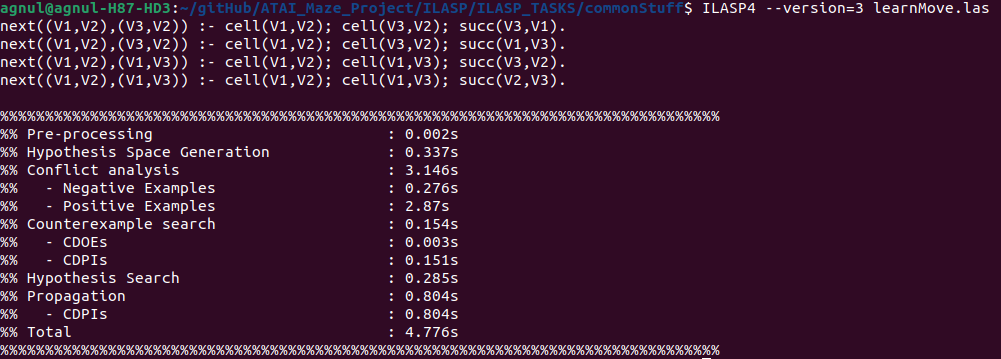
\includegraphics[scale=0.5]{img/learnMoveAdj.png}
	\caption{Learned rules - adjacent move}\label{fig:asd}
\end{figure}

\newpage
\subsubsection{Learning to walk on cells without obstacles}
The next step is to consider obstacles on the grid, as discussed in the Introduction part of the report. Here the goal is to find a new normal rule that represent the concet of a "valid move", in a cell without obstacles.
Initially, a maze is defined, this is the same maze used by my companions for our work.
This is the task written for the purpose:
\newpage

\begin{lstlisting}[language=Prolog]
%%%%%%%%%%%%%%%%%%%%%%%%%%%%%%learn how to move on cells without obstacles
row(1..5).
col(1..5).

obstacle(1,2).
obstacle(2,2).
obstacle(3,2).
obstacle(3,3).
obstacle(4,3).
obstacle(4,4).
obstacle(3,4).
obstacle(2,4).
obstacle(1,4).
obstacle(1,5).
obstacle(5,1).

start(1,1).
goal(5,5).

%%%%%%%%%%%%%%

cell(X,Y) :- row(X), col(Y).

succ(0,1).
succ(X, X+1) :- cell(X,_).

%PATHS ADJACENTS (learned from previous ilasp task)
next((V1,V2),(V3,V2)) :- cell(V1,V2), cell(V3,V2), succ(V3,V1).
next((V1,V2),(V3,V2)) :- cell(V1,V2), cell(V3,V2), succ(V1,V3).
next((V1,V2),(V1,V3)) :- cell(V1,V2), cell(V1,V3), succ(V3,V2).
next((V1,V2),(V1,V3)) :- cell(V1,V2), cell(V1,V3), succ(V2,V3).


%%%%%%%%%%%%%%%%%%%%%%%%%%%%%SEARCH_SPACE + EXAMPLES

#pos(po, {nextLegit((1,1),(2,1))}, {}).
#pos(po2, {nextLegit((4,1),(4,2))}, {}).

%no movement on obstacles
#neg(a, {nextLegit((1,1),(1,2))}, {}).
#neg(av, {nextLegit((3,2),(4,2))}, {}).
#neg(af, {nextLegit((1,2),(1,1))}, {}).
#neg(b, {nextLegit((4,1),(5,1))}, {}).
#neg(g, {nextLegit((3,3),(2,3))}, {}).

#modeb(1, next((var(r), var(c)), (var(r), var(c)))).
#modeb(2, obstacle(var(r), var(c))).
#modeh(1, nextLegit((var(r), var(c)), (var(r), var(c)))).

#maxv(3).
\end{lstlisting}
In the code the rules learned previously have been inserted and used in the search space. 
Negative examples shows that no movement is possible TO obstacles and FROM obstacles, this 2 casistics are important for a correct learning.
At \ref{fig:asd2} the output of the script, with the learned rules, ILASP actually learned this new "nextLegit" predicate that represent the concept of a valid move: a move from (or to) cells without obstacles.

NB: this is equivalent to the "move" predicate learned by my companions.
\begin{figure}
	\centering
	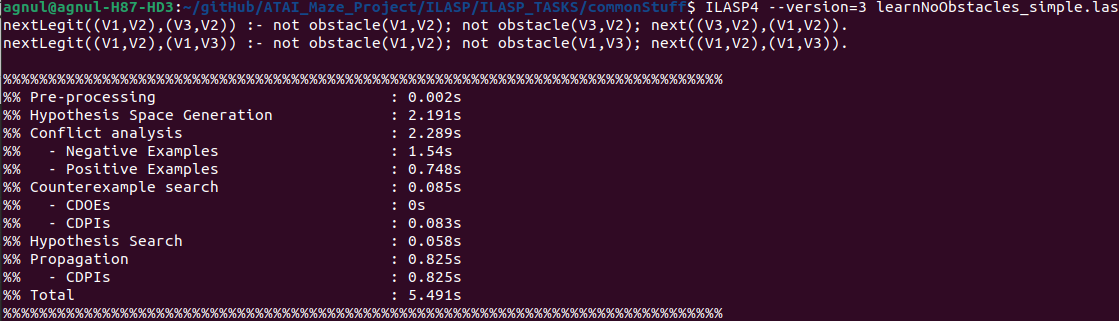
\includegraphics[scale=0.45]{img/learn_noObstacles.png}
	\caption{Learned rules - avoid obstacles}\label{fig:asd2}
\end{figure}


\newpage
It's interesting to see that, setting 3 variables in the language bias, ilasp learned just 2 rules: it considers the cases when near cells share the same horizontal or vertical direction. 
Probably, I would have write 4 rules using 4 different variables in a naive way, considering the "4 directions adjacency", but this tool finds a more compact solution.
\subsubsection{using this rules to define an ASP model}
having this rules in hand now is possible to define a model that solves our problem. Learned rules are reported exactly as they were on the ILASP scripts output. Some pieces are missing: some other rules need to be defined but they are quite intiuitive at this point. The maze reported on the encoding is the same used for the ilasp task.
 
 \newpage
\begin{lstlisting}[language=Prolog]
	%MODEL THAT SOLVES PROBLEM OF PATHFINDING IN THE GRID
	row(1..5).
	col(1..5).
	
	obstacle(1,2).
	obstacle(2,2).
	obstacle(3,2).
	obstacle(4,4).
	obstacle(3,4).
	obstacle(2,4).
	obstacle(1,4).
	obstacle(1,5).
	obstacle(5,1).
	
	start(1,1).
	goal(2,5).
	
	%for each position define cell pred.
	cell(X,Y) :- row(X), col(Y).
	
	%FIND A PATH FROM START
	move(0,0,X,Y) :- start(X,Y).
	%for each "move" find another linked to it that is a legit move!
	1{move(X,Y,X1,Y1): nextLegit((X,Y), (X1,Y1))}1:- move(_,_, X,Y), not goal(X,Y).
	
	succ(0,1).
	succ(X, X+1) :- cell(X,_).
	
	%LEARNED BY ILASP, move on adj cells.
	next((V1,V2),(V3,V2)) :- cell(V1,V2), cell(V3,V2), succ(V3,V1).
	next((V1,V2),(V3,V2)) :- cell(V1,V2), cell(V3,V2), succ(V1,V3).
	next((V1,V2),(V1,V3)) :- cell(V1,V2), cell(V1,V3), succ(V3,V2).
	next((V1,V2),(V1,V3)) :- cell(V1,V2), cell(V1,V3), succ(V2,V3).
	
	%LEARNED BY ILASP, move on adj cells. without obstacles
	nextLegit((V1,V2),(V3,V2)) :- not obstacle(V1,V2); not obstacle(V3,V2); next((V3,V2),(V1,V2)).
	nextLegit((V1,V2),(V1,V3)) :- not obstacle(V1,V2); not obstacle(V1,V3); next((V1,V2),(V1,V3)).
	
	%ON GOAL POSITION STOP
	:- goal(X,Y), not move(_,_, X,Y).
	
	#show move/4.
\end{lstlisting}

at \ref{fig:asd3} the execution of "clingo" command on this model is shown: the path is represented by the chaning "move" predicate.

\newpage
\begin{figure}
	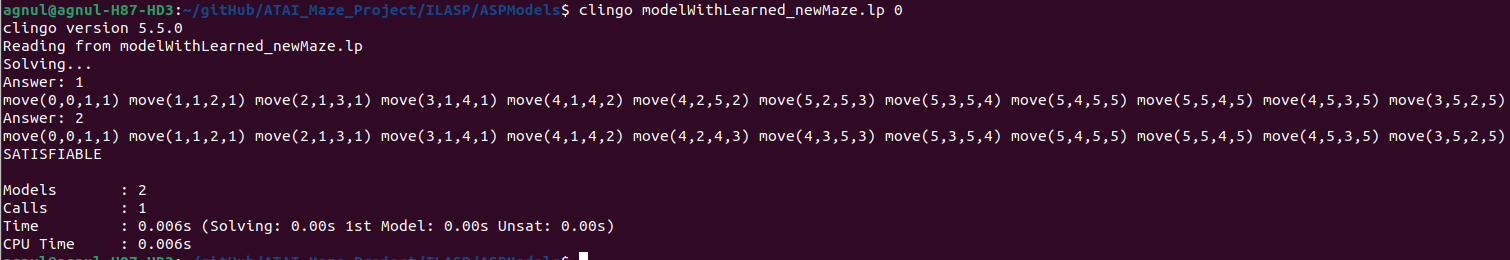
\includegraphics[scale=0.3]{img/outputModel_newMaze.png}
	\caption{Path found on the grid}\label{fig:asd3}
\end{figure}

\subsubsection{performance test - scalability}
The work done with ilasp shows clearly this fact: the time complexity doesn't scale well with respect to the search space dimension. In fact, when trying to learn the "move to adjacent cells AND without obstacles" (the 2 tasks on the same scrit) compexity costs exploded "simply" for the insertion of the predicate "obstacle". (for a total of 6 predicates in the search space). it is quite evident that a sort of exponential trend is in place and here I will like to do a specific test to demonstrate this.

Using the "learn to walk on adjacent cells" ilasp script I tried to augment the search space and see time needed for computation, the augmenting has been done insertig other predicates in language bias, modyfing language bias to insert more "usage" of the same predicate, eliminating the "positive" and "anti-reflexing" options on language bias. After that, an analysis on computation time vs search space dimension (measured as the size of rules in the search space) has been conducted, at \ref{fig:asd4} the graphical results, the blue points are the instantes of the benchmarks. Interestingly other tests conducted with a searh space grater than 200 lead to huge times like 2 hours.

The grow shows an evident simil-exponential trend, especially the steep from the "57 seconds" point to the "200" one.
\newpage

\begin{figure}
	\centering
	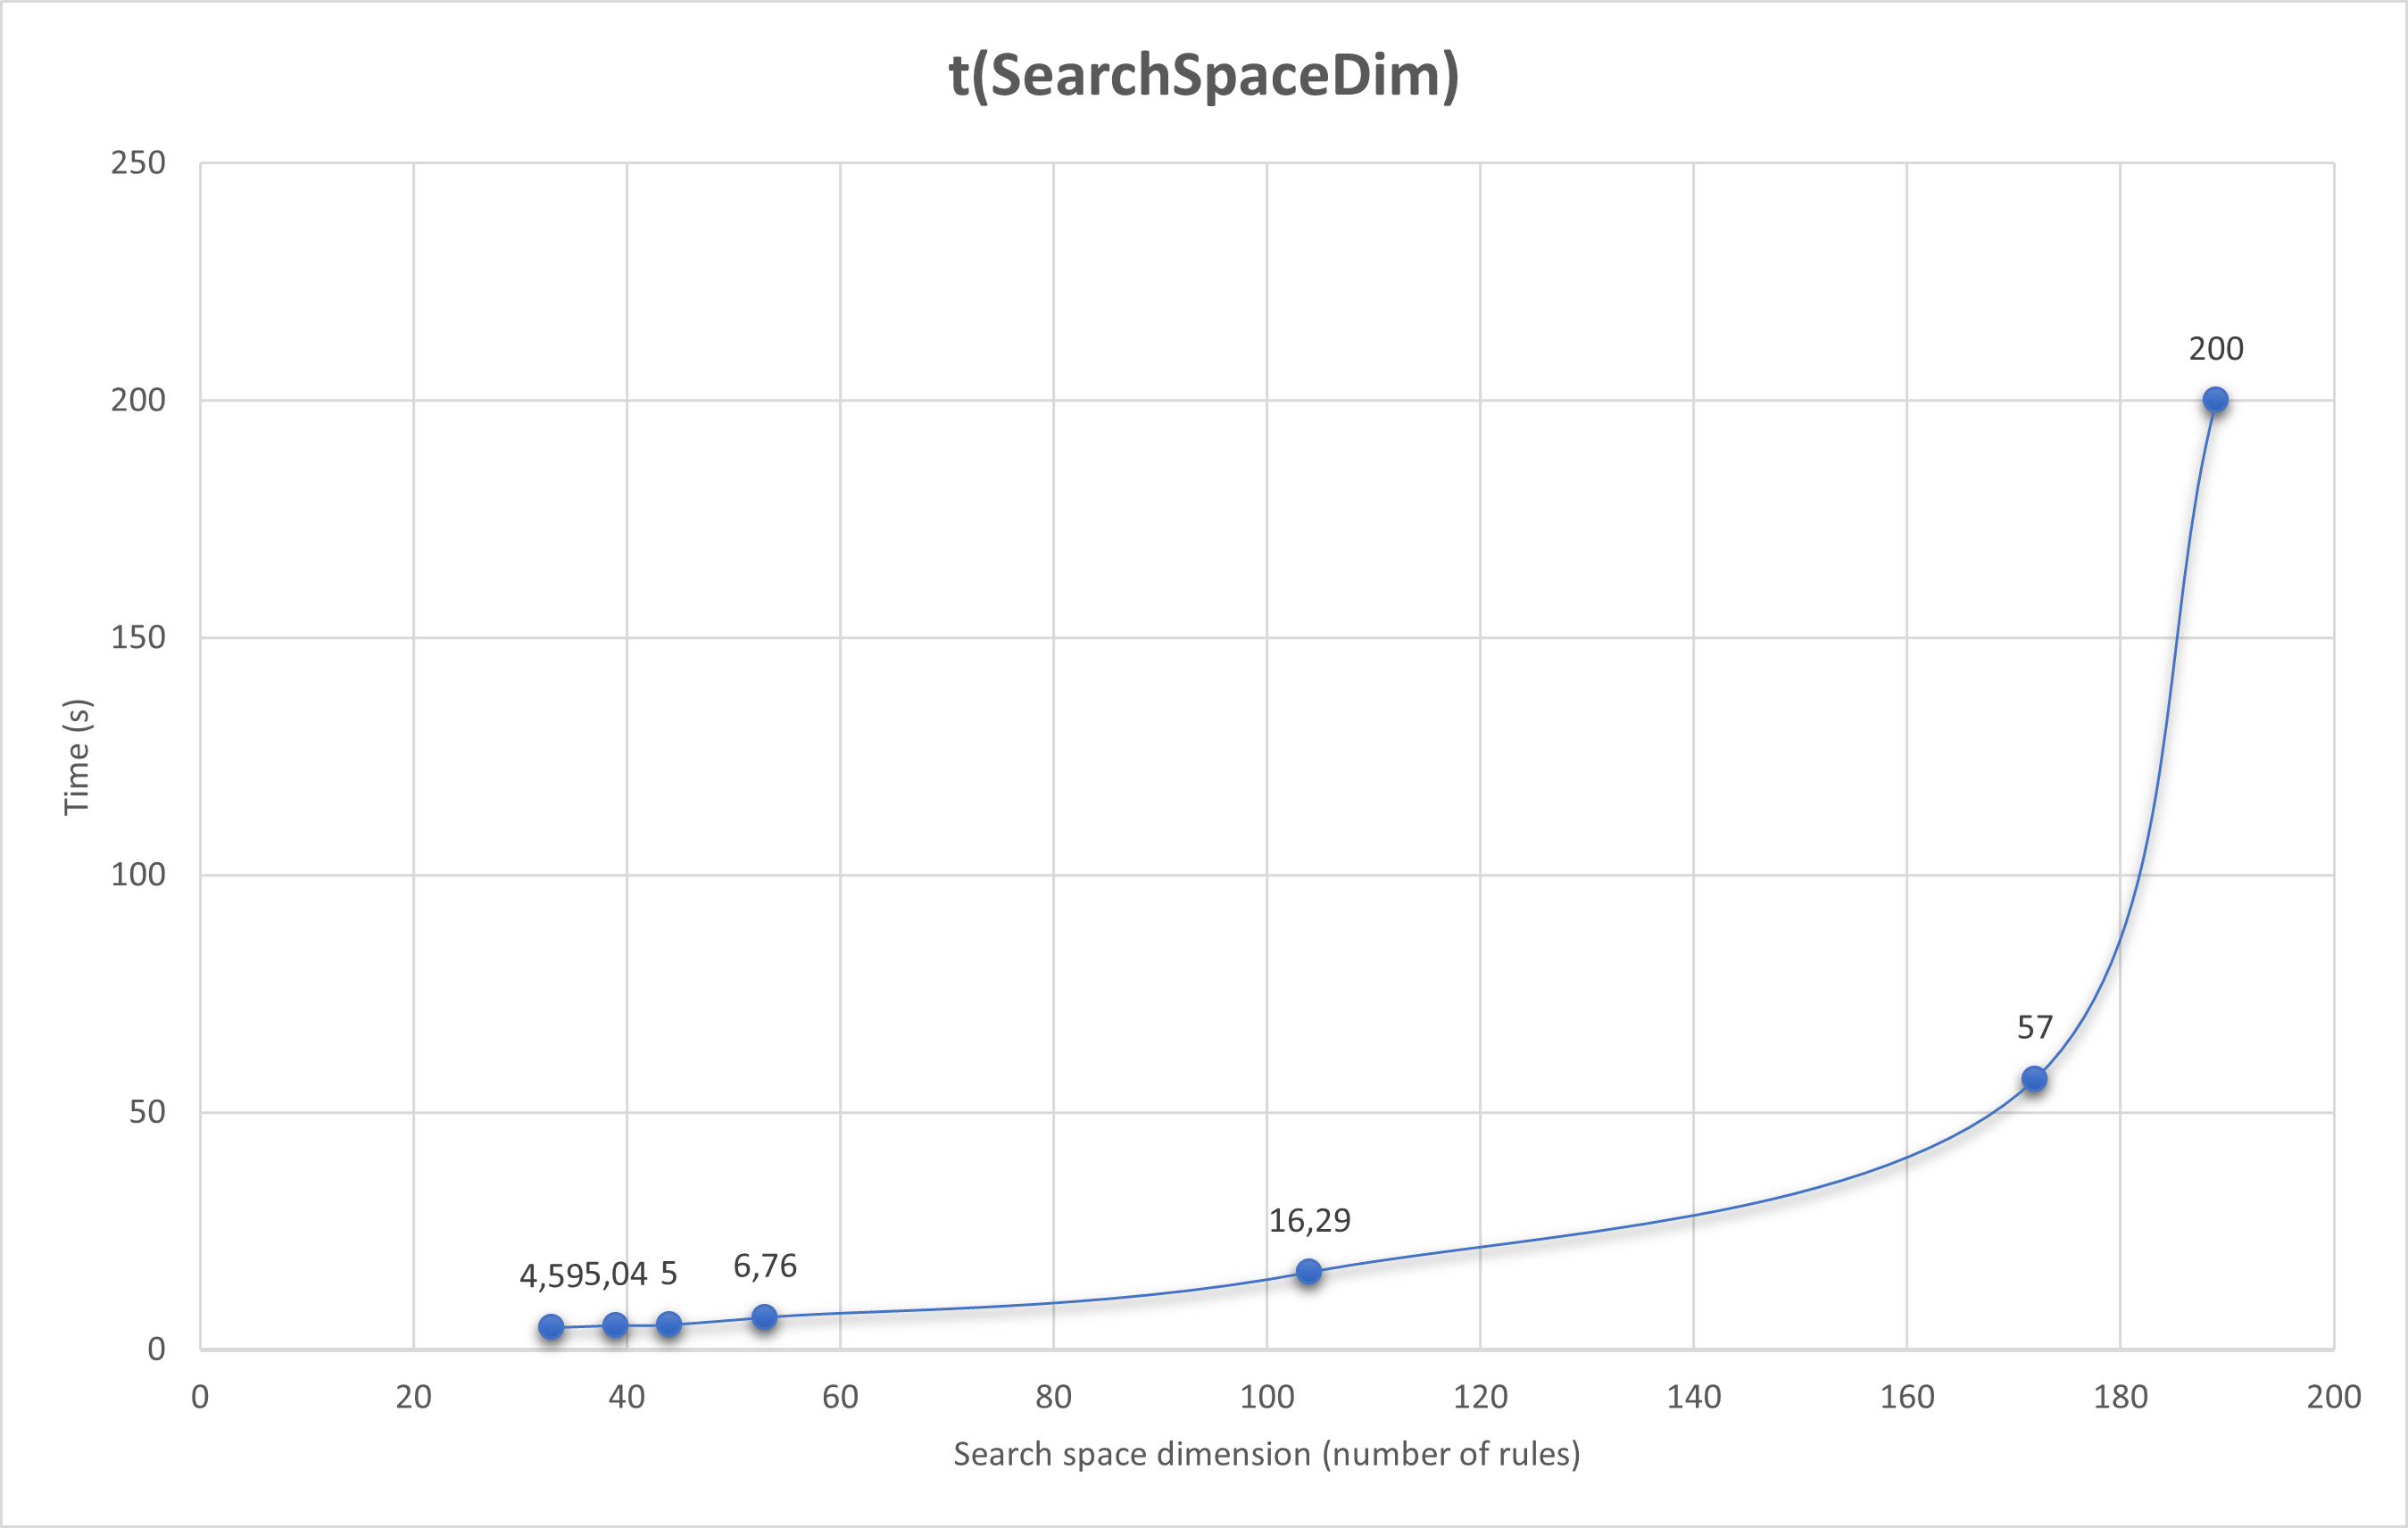
\includegraphics[scale=0.7]{img/GraphTimes.png}
	\caption{performance test result}\label{fig:asd4}
\end{figure}



\newpage
\section{Performance comparison}\label{sec:perf}


{\rowcolors{2}{gray!50!}{}
\begin{center}
    \begin{tabular}{ |l|c|c|c| } 
        \hline
        Task & \textbf{HYPER} & \textbf{Metagol} & \textbf{ILASP} \\ \hline
        \texttt{adjacent/2} & 175.884 & 0.056 & 4.767 \\ 
        \texttt{move/2} & 0.063 & 0.047 & 5.343 \\ 
        \texttt{move/2} (\(7*7\) grid) & INSERT & 0.054 & INSERT \\ 
        \texttt{reach/3} & 1.577 & 0.027 & NA \\ 
        \texttt{move/2} and \texttt{reach/3} & 16.585 & 0.848 & NA \\ 
        \hline
    \end{tabular}
\end{center}
}

\end{document}
